\chapter{强化学习和序列建模}

许多现实世界问题并不是一次性完成预测，而是要求行动者持续观察环境、采取行动并接收反馈。环境动态可能未知，行动的影响也可能延迟出现，因此模型需要在连续交互中学习长期有效的行为。

强化学习（Reinforcement Learning, RL）作为一种独特的机器学习范式，为解决这类动态、不确定环境下的序列决策问题提供了强大的框架。它通过让智能体在环境中不断试错和学习，从经验中发现最优的行动策略，以最大化长期累积奖励。这种学习方式与人类学习过程中的”试错”和”反馈”机制高度相似。

本章讨论强化学习的核心概念、马尔可夫决策过程，以及基于价值和基于策略的经典方法。重点是理解状态、行动、奖励和长期回报如何共同定义一个序列决策问题，并判断 AI 生成的强化学习方案是否允许安全、有效的验证。

\begin{chapterguide}
\begin{itemize}
  \item 用状态、行动、奖励、策略和价值函数把一个序列决策问题表述为马尔可夫决策过程；
  \item 区分基于模型与无模型、基于价值与基于策略、同策略与异策略等算法类别；
  \item 说明价值迭代、Q-learning、SARSA、DQN 和策略梯度的工作原理与适用条件；
  \item 认识强化学习结果对超参数、随机种子和训练长度的敏感性，并以可靠的方式报告结果；
  \item 判断奖励函数、安全约束和比较对象是否被合理定义。
\end{itemize}
\end{chapterguide}

\section{强化学习基本概念}
在“机器学习基础知识”章节中，我们已经简要介绍了强化学习的基本组成部分。现在，我们将对这些概念进行更深入的阐述，为理解后续算法奠定基础。

\subsection{智能体（Agent）与环境（Environment）}
强化学习的核心是智能体与环境之间的持续交互。
\begin{itemize}
    \item \textbf{智能体（Agent）：} 是学习者和决策者。它在环境中感知状态，选择行动，并从环境的响应中学习。
    \item \textbf{环境（Environment）：} 是智能体所处的外部世界。它接收智能体的行动，根据其内部动力学演化到新的状态，并给予智能体奖励。
\end{itemize}
这种交互是一个循环过程：智能体观察状态 $\to$ 智能体选择行动 $\to$ 环境给出奖励和新状态 $\to$ 智能体再次观察新状态，如此往复。

\begin{figure}[H]
  \centering
  \begin{tikzpicture}[font=\small, >=Stealth, b/.style={draw, rounded corners, minimum width=30mm, minimum height=11mm, align=center}]
\node[b, fill=blue!15] (a) at (0,1.6) {智能体（Agent）\\策略 $\pi(a|s)$};
\node[b, fill=green!15] (e) at (0,-1.6) {环境（Environment）\\状态转移 $P(s'|s,a)$};
\draw[->, thick] (a.east) -- ++(1.6,0) |- node[pos=0.25, right] {行动 $A_t$} (e.east);
\draw[->, thick] (e.west) -- ++(-1.9,0) |- node[pos=0.25, left, align=right] {新状态 $S_{t+1}$\\奖励 $R_{t+1}$} (a.west);
\end{tikzpicture}

  \caption{智能体与环境的交互循环}
  \label{fig:ch10_orig1}
\end{figure}

\subsection{状态（State）、行动（Action）与奖励（Reward）}
\begin{itemize}
    \item \textbf{状态（State, $s$）：} 环境在某一时刻的完整描述，包含了智能体做出决策所需的所有信息。例如，在下棋游戏中，棋盘上所有棋子的位置构成一个状态；在机器人导航中，机器人的位置、方向和周围地图信息构成一个状态。状态可以是离散的（如棋盘格子）也可以是连续的（如机器人的精确坐标）。
    \item \textbf{行动（Action, $a$）：} 智能体在给定状态下可以执行的操作。行动可以是离散的（如向左、向右、跳跃）也可以是连续的（如机器人关节的旋转角度）。
    \item \textbf{奖励（Reward, $r$）：} 环境对智能体行动的即时反馈。奖励是一个标量值，用于衡量智能体在当前状态下采取某个行动的好坏。智能体的最终目标是最大化其累积奖励（通常是折扣累积奖励）。奖励通常是稀疏的，即只有在达到特定目标或发生特定事件时才会获得显著的奖励或惩罚。
\end{itemize}

\subsection{策略（Policy）}
\textbf{策略（Policy, $\pi$）}是智能体的行为准则，它定义了智能体在给定状态下选择哪个行动。策略可以表示为：
\begin{itemize}
    \item \textbf{确定性策略（Deterministic Policy）：} $\pi(s) = a$，表示在状态 $s$ 下总是选择行动 $a$。
    \item \textbf{随机性策略（Stochastic Policy）：} $\pi(a|s) = P(A=a|S=s)$，表示在状态 $s$ 下选择行动 $a$ 的概率。随机性策略有助于探索环境，避免陷入局部最优。
\end{itemize}
强化学习的目标就是学习一个最优策略 $\pi^*$，使得智能体能够获得最大的长期累积奖励。

\begin{figure}[H]
  \centering
  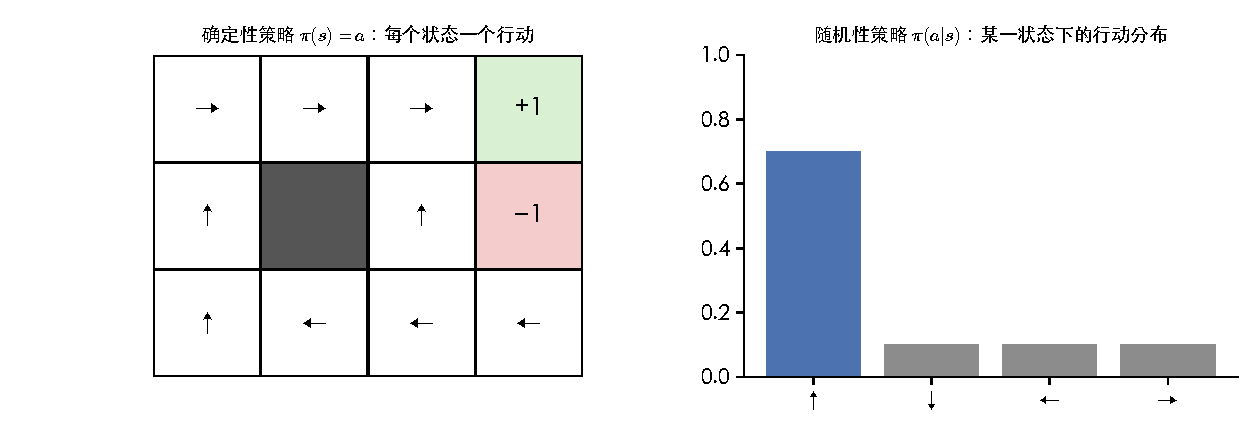
\includegraphics[width=0.9\textwidth]{figures/chapter10/grid_policy.pdf}
  \caption{确定性策略（左，4×3 网格世界中由价值迭代得到的最优策略）与随机性策略（右，示意）}
  \label{fig:ch10_orig2}
\end{figure}

\subsection{价值函数（Value Function）}
价值函数用于衡量在给定状态下或在给定状态下采取某个行动后，智能体能够获得的未来累积奖励的期望。它们帮助智能体评估不同状态或行动的“好坏”。
\begin{itemize}
    \item \textbf{状态价值函数（State-Value Function, $V^\pi(s)$）：} 表示从状态 $s$ 开始，并遵循策略 $\pi$ 能够获得的预期累积奖励。
    $$ V^\pi(s) = E_\pi [G_t | S_t = s] = E_\pi \left[ \sum_{k=0}^{\infty} \gamma^k R_{t+k+1} | S_t = s \right] $$
    \item \textbf{行动价值函数（Action-Value Function, $Q^\pi(s, a)$）：} 表示在状态 $s$ 下采取行动 $a$，然后遵循策略 $\pi$ 能够获得的预期累积奖励。
    $$ Q^\pi(s, a) = E_\pi [G_t | S_t = s, A_t = a] = E_\pi \left[ \sum_{k=0}^{\infty} \gamma^k R_{t+k+1} | S_t = s, A_t = a \right] $$
\end{itemize}
其中 $G_t$ 是从时刻 $t$ 开始的折扣累积奖励（回报），$\gamma \in [0, 1]$ 是折扣因子，用于平衡即时奖励和未来奖励的重要性。$\gamma$ 越大，未来奖励在计算中占的比重越大。

\begin{figure}[H]
  \centering
  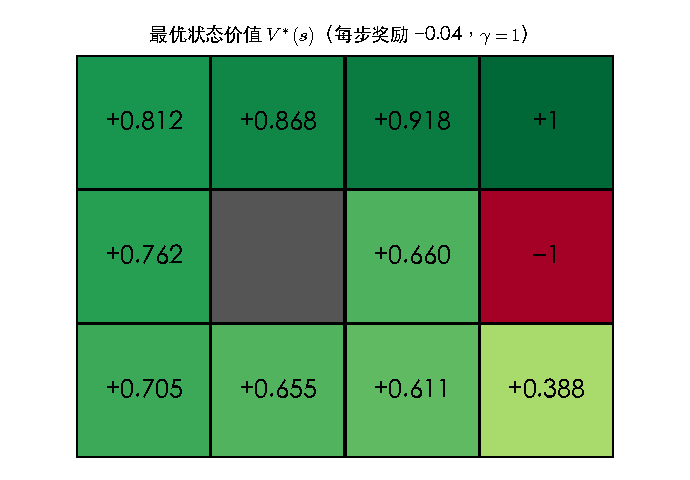
\includegraphics[width=0.55\textwidth]{figures/chapter10/grid_values.pdf}
  \caption[4×3 网格世界中由价值迭代计算得到的最优状态价值]{4×3 网格世界中由价值迭代计算得到的最优状态价值（代码见 \texttt{code/figures/concept\_figures.py}）}
  \label{fig:ch10_orig3}
\end{figure}

\subsection{模型（Model）}
在强化学习中，“模型”指的是智能体对环境动态的理解。
\begin{itemize}
    \item \textbf{基于模型的强化学习（Model-Based RL）：} 智能体尝试学习或已知环境的动力学模型，即状态转移概率 $P(s'|s, a)$ 和奖励函数 $R(s, a, s')$. 学习到模型后，智能体可以进行“规划”（Planning），通过模拟环境来预测行动的后果，从而推导出最优策略。
    \item \textbf{无模型强化学习（Model-Free RL）：} 智能体不尝试学习环境模型，而是直接从与环境的交互经验中学习策略或价值函数。这种方法适用于环境模型复杂或未知的情况。
\end{itemize}

\section{马尔可夫决策过程（Markov Decision Process, MDP）}
马尔可夫决策过程（MDP）是强化学习的数学基础，它提供了一个形式化的框架来描述强化学习问题。一个MDP是一个五元组 $(S, A, P, R, \gamma)$：
\begin{itemize}
    \item $S$: 有限状态的集合。
    \item $A$: 有限行动的集合。
    \item $P(s'|s, a)$: 状态转移概率函数，表示在状态 $s$ 采取行动 $a$ 后，转移到下一个状态 $s'$ 的概率。这满足\textbf{马尔可夫性质（Markov Property）}：下一状态仅取决于当前状态和当前行动，而与之前的状态和行动无关。
    \item $R(s, a, s')$: 奖励函数，表示从状态 $s$ 采取行动 $a$ 转移到状态 $s'$ 时获得的即时奖励。简化情况下，也可以是 $R(s, a)$ 或 $R(s')$.
    \item $\gamma$: 折扣因子，$\gamma \in [0, 1)$。
\end{itemize}

\subsection{MDP 经典示例：网格世界（Grid World）}
为了直观理解 MDP，我们可以看一个简单的 $4 \times 3$ 网格环境。
\begin{figure}[H]
  \centering
  \resizebox{0.95\textwidth}{!}{\begin{tikzpicture}[font=\small, >=Stealth]
\foreach \c in {0,...,3} \foreach \r in {0,...,2} \draw (1.2*\c,1.2*\r) rectangle ++(1.2,1.2);
\fill[gray!70] (1.2,1.2) rectangle ++(1.2,1.2); \node[white] at (1.8,1.8) {墙};
\fill[green!25] (3.6,2.4) rectangle ++(1.2,1.2); \node at (4.2,3.0) {$+1$};
\fill[red!20] (3.6,1.2) rectangle ++(1.2,1.2); \node at (4.2,1.8) {$-1$};
\node at (0.6,0.6) {起点};
\draw[->, thick, blue] (0.6,1.9) -- node[right, font=\scriptsize] {0.8} (0.6,2.8);
\draw[->, thick, blue!50] (0.6,1.9) -- node[above, font=\scriptsize] {0.1} (0.1,1.9);
\draw[->, thick, blue!50] (0.6,1.9) -- node[above, font=\scriptsize] {0.1} (1.1,1.9);
\node[anchor=west, align=left, font=\scriptsize] at (5.2,1.8) {状态：11 个可到达格子\\行动：上、下、左、右\\转移：以 0.8 的概率按意图移动，\\\quad 各以 0.1 的概率偏向两侧；\\\quad 撞墙或出界则留在原地\\奖励：每走一步 $-0.04$，\\\quad 到达终点获得 $+1$ 或 $-1$};
\end{tikzpicture}
}
  \caption{4×3 网格世界：状态、行动、随机转移与奖励}
  \label{fig:ch10_orig4}
\end{figure}

\subsection{贝尔曼方程（Bellman Equations）}
贝尔曼方程是MDP中的核心概念，它以递归的方式定义了价值函数。它表达了当前状态的价值与其可能达到的下一个状态的价值之间的关系。

\textbf{状态价值函数的贝尔曼期望方程：}
$$ V^\pi(s) = \sum_{a \in A} \pi(a|s) \sum_{s' \in S} P(s'|s, a) [R(s, a, s') + \gamma V^\pi(s')] $$
这表示在状态 $s$ 下的价值，等于遵循策略 $\pi$ 后所有可能行动的价值，再加权平均。

\textbf{行动价值函数的贝尔曼期望方程：}
$$ Q^\pi(s, a) = \sum_{s' \in S} P(s'|s, a) [R(s, a, s') + \gamma V^\pi(s')] $$
$$ V^\pi(s) = \sum_{a \in A} \pi(a|s) Q^\pi(s, a) $$
通过这两个方程，可以相互推导 $V^\pi(s)$ 和 $Q^\pi(s, a)$。

\textbf{贝尔曼最优方程（Bellman Optimality Equations）：}
为了找到最优策略 $\pi^*$，我们需要找到最优价值函数 $V^*(s)$ 和 $Q^*(s, a)$。最优价值函数是所有可能策略中能达到的最大价值：
$$ V^*(s) = \max_{a \in A} \sum_{s' \in S} P(s'|s, a) [R(s, a, s') + \gamma V^*(s')] $$
$$ Q^*(s, a) = \sum_{s' \in S} P(s'|s, a) [R(s, a, s') + \gamma \max_{a'} Q^*(s', a')] $$
一旦我们获得了最优 $Q^*$ 函数，最优策略 $\pi^*$ 就可以通过在每个状态选择使得 $Q^*$ 最大的行动来确定：
$$ \pi^*(s) = \arg\max_{a \in A} Q^*(s, a) $$

\section{强化学习算法分类}
强化学习算法可以从不同维度进行分类：


\begin{figure}[H]
  \centering
  \resizebox{\textwidth}{!}{\begin{tikzpicture}[font=\scriptsize, >=Stealth, level distance=13mm,
  every node/.style={draw, rounded corners, align=center, fill=gray!8, minimum height=7mm},
  level 1/.style={sibling distance=78mm}, level 2/.style={sibling distance=33mm}]
\node[fill=blue!15] {强化学习算法}
  child {node[fill=green!15] {基于模型\\（已知或学习环境模型）}
    child {node {动态规划\\价值迭代、策略迭代}}
    child {node {学习模型并规划\\如 Dyna、MPC 类方法}}}
  child {node[fill=orange!15] {无模型\\（直接从交互中学习）}
    child {node {基于价值\\Q-Learning、SARSA、DQN}}
    child {node {基于策略\\REINFORCE}}
    child {node {Actor-Critic\\A2C、PPO、SAC}}};
\node[draw=none, fill=none] at (0,-4.3) {另一个维度：同策略（SARSA、REINFORCE、PPO）与异策略（Q-Learning、DQN、SAC）};
\end{tikzpicture}
}
  \caption{强化学习算法的主要分类}
  \label{fig:ch10_orig5}
\end{figure}

\subsection{基于模型（Model-Based）与无模型（Model-Free）}
\begin{itemize}
    \item \textbf{基于模型（Model-Based）算法：} 智能体要么已知环境的模型（即状态转移概率 $P$ 和奖励 $R$），要么在学习过程中估计这些模型。一旦模型已知或学到，智能体就可以通过“规划”来找出最优策略，例如使用动态规划（Dynamic Programming）。
        \begin{itemize}
            \item \textbf{优点：} 样本效率高（学习速度快），因为可以通过模型进行模拟。
            \item \textbf{缺点：} 学习环境模型本身可能很困难或计算量大；如果模型不准确，可能导致次优决策。
        \end{itemize}
    \item \textbf{无模型（Model-Free）算法：} 智能体不学习环境模型，而是直接从经验中学习价值函数或策略。它们通过与环境的真实交互来更新模型。
        \begin{itemize}
            \item \textbf{优点：} 不需要知道环境模型，适用于模型复杂或无法获取的情况。
            \item \textbf{缺点：} 样本效率通常较低，需要大量的试错经验。
        \end{itemize}
\end{itemize}

\subsection{价值学习（Value-Based）与策略学习（Policy-Based）}
\begin{itemize}
    \item \textbf{价值学习（Value-Based）算法：} 这类算法的目标是学习一个最优的价值函数（$V^*$ 或 $Q^*$），然后通过这个价值函数来推导出最优策略。例如，Q-Learning 和 SARSA。
        \begin{itemize}
            \item \textbf{优点：} 通常在离散状态和动作空间中表现良好。
            \item \textbf{缺点：} 难以直接处理连续动作空间；在动作空间维度很高时，Q值表的存储和学习变得困难。
        \end{itemize}
    \item \textbf{策略学习（Policy-Based）算法：} 这类算法直接学习策略本身，即学习一个函数来直接输出在给定状态下应该采取的行动，或采取不同行动的概率。例如，策略梯度（Policy Gradient）方法。
        \begin{itemize}
            \item \textbf{优点：} 能够自然地处理连续动作空间；能够学习随机性策略。
            \item \textbf{缺点：} 通常收敛速度较慢，容易陷入局部最优。
        \end{itemize}
    \item \textbf{演员-评论家（Actor-Critic）算法：} 结合了价值学习和策略学习的优点。一个“演员（Actor）”负责学习策略并采取行动，一个“评论家（Critic）”负责学习价值函数并评估演员的行动，然后用这个评估来指导演员改进策略。
\end{itemize}

\subsection{同策略（On-Policy）与异策略（Off-Policy）}
\begin{itemize}
    \item \textbf{同策略（On-Policy）算法：} 智能体用于学习和改进策略的经验数据，是从\textbf{当前策略}（即正在学习和改进的策略）中获得的。也就是说，智能体执行的策略和它学习的策略是同一个。例如 SARSA。
        \begin{itemize}
            \item \textbf{优点：} 简单直接，通常更稳定。
            \item \textbf{缺点：} 每次策略更新后，旧的经验数据就无法再被用来学习新策略，样本效率可能较低。
        \end{itemize}
    \item \textbf{异策略（Off-Policy）算法：} 智能体用于学习和改进策略的经验数据，可以是从\textbf{另一个策略}（行为策略，Behavior Policy）中获得的，或者来自历史数据。这允许智能体更自由地探索环境，并且可以重用旧的经验数据。例如 Q-Learning 和 DQN。
        \begin{itemize}
            \item \textbf{优点：} 样本效率高，可以从历史数据中学习；有助于更充分地探索环境。
            \item \textbf{缺点：} 通常更复杂，收敛性可能不如同策略算法稳定。
        \end{itemize}
\end{itemize}

\section{核心算法的工作原理}
本节将介绍几种具有代表性的强化学习算法，并提供Python代码示例。

\subsection{基于模型的动态规划：价值迭代（Value Iteration）}
价值迭代是一种基于模型的动态规划算法，它通过迭代地更新状态价值函数 $V(s)$，使其收敛到最优状态价值函数 $V^*(s)$。一旦 $V^*(s)$ 收敛，就可以从中推导出最优策略。价值迭代的关键在于使用贝尔曼最优方程作为更新规则。

算法流程：
\begin{enumerate}
    \item \textbf{初始化：} 随机初始化所有状态的价值 $V(s)$ (或全部设为0)。
    \item \textbf{迭代更新：} 重复以下步骤直到 $V(s)$ 收敛：
    对于每个状态 $s \in S$：
    $$ V_{k+1}(s) = \max_{a \in A} \sum_{s' \in S} P(s'|s, a) [R(s, a, s') + \gamma V_k(s')] $$
    \item \textbf{提取最优策略：} 当 $V(s)$ 收敛到 $V^*(s)$ 后，最优策略 $\pi^*(s)$ 可以通过在每个状态 $s$ 选择使等式右侧最大化的行动 $a$ 来确定：
    $$ \pi^*(s) = \arg\max_{a \in A} \sum_{s' \in S} P(s'|s, a) [R(s, a, s') + \gamma V^*(s')] $$
\end{enumerate}
价值迭代是收敛的，并且能找到最优策略。它要求已知环境模型（即 $P(s'|s, a)$ 和 $R(s, a, s')$）。

\paragraph{实现：小型网格世界}
我们将在一个小型的确定性网格世界中演示价值迭代。智能体从任意位置开始，目标是到达目标方块，避开陷阱。

完整代码见 \texttt{code/ch10\_rl/demos.py}（\texttt{python demos.py gridworld}）。在一个 $4\times4$ 的确定性网格中，右上角为目标（奖励 $+1$），其下方为陷阱（奖励 $-1$），其余每走一步奖励 $-0.04$，折扣因子 $\gamma=0.9$。价值迭代 4 次即收敛，得到的最优策略为：
\begin{center}
\begin{tabular}{cccc}
$\rightarrow$ & $\rightarrow$ & $\rightarrow$ & G \\
$\uparrow$ & $\uparrow$ & $\uparrow$ & X \\
$\uparrow$ & $\uparrow$ & $\uparrow$ & $\leftarrow$ \\
$\uparrow$ & $\uparrow$ & $\uparrow$ & $\uparrow$ \\
\end{tabular}
\end{center}
可以看到，陷阱正下方的格子选择向左绕行，而不是直接向上经过陷阱——这正是价值函数把未来风险“传播”回当前决策的结果。
价值迭代是一种离线规划算法，它在知道环境模型的情况下，通过迭代地更新价值函数，最终找到最优策略。它保证收敛到全局最优，但其计算复杂度随状态空间和动作空间的增大而迅速增加，因此主要适用于小规模的MDP问题。

\subsection{无模型学习：Q-Learning}
Q-学习（Q-Learning）是一种无模型的强化学习算法，它不需要预先知道环境的状态转移概率和奖励函数。它直接学习最优的行动价值函数 $Q^*(s, a)$。Q-学习是异策略（Off-Policy）的，这意味着它可以从任何探索策略中学习最优策略，而不仅仅是当前正在优化的策略。

Q-学习的核心是其迭代更新规则（贝尔曼最优方程的蒙特卡洛采样版本）：
$$ Q(s_t, a_t) \leftarrow Q(s_t, a_t) + \alpha [r_{t+1} + \gamma \max_{a} Q(s_{t+1}, a) - Q(s_t, a_t)] $$
在每个时间步 $t$：
\begin{enumerate}
    \item 智能体在状态 $s_t$ 采取行动 $a_t$（通常通过 $\epsilon$-贪婪策略选择）。
    \item 环境返回即时奖励 $r_{t+1}$ 和下一个状态 $s_{t+1}$。
    \item 智能体使用这个经验 $(s_t, a_t, r_{t+1}, s_{t+1})$ 更新 $Q(s_t, a_t)$。更新时，它使用 $Q(s_{t+1}, a)$ 的最大值来估计未来的最优回报，这使得 Q-Learning 是异策略的。
\end{enumerate}
Q-学习的收敛性依赖于一些条件，例如所有状态-动作对必须被无限次访问（通过足够的探索），以及学习率 $\alpha$ 逐渐衰减。

\paragraph{实现：迷宫寻路问题}
我们将使用一个简单的迷宫寻路问题来演示Q-学习。智能体的目标是从起点（S）走到终点（G），并避开障碍物（墙壁）。

\textbf{迷宫环境设置：}
我们定义一个简单的4x4迷宫，其中：
\begin{itemize}
    \item 'S': 起点
    \item 'G': 终点（奖励 +100）
    \item 'W': 墙壁（惩罚 -100，回到原位）
    \item '.': 空地（每走一步小惩罚 -1）
\end{itemize}
智能体可以向上、下、左、右四个方向移动。

完整代码见 \texttt{demos.py maze}。迷宫布局为（S 起点、G 终点、W 墙）：\texttt{S.W.}\,/\,\texttt{..W.}\,/\,\texttt{....}\,/\,\texttt{W..G}。以 $\alpha=0.1$、$\gamma=0.95$、$\epsilon=0.1$ 训练 500 回合，前 50 回合的平均回报为 65.0，最后 50 回合为 76.4；学到的贪心策略用 6 步从起点到达终点，绕开了两堵墙。
Q-学习通过迭代更新Q值表，能够让智能体在没有明确环境模型的情况下学习到最优策略。它在状态和动作空间较小的离散决策问题中表现良好。然而，当状态空间或动作空间非常大时，Q-表会变得非常庞大，难以存储和计算。这时，需要使用更复杂的强化学习方法，例如结合神经网络来近似Q函数（如深度Q网络DQN），这些内容将在后续章节中深入探讨。


\subsection{无模型学习：SARSA}
SARSA（State-Action-Reward-State-Action）是另一种无模型的强化学习算法，与Q-学习非常相似，但它是\textbf{同策略（On-Policy）}的。这意味着SARSA在更新 $Q(s_t, a_t)$ 时，使用的是当前策略在下一个状态 $s_{t+1}$ 下实际选择的行动 $a_{t+1}$ 所对应的 $Q(s_{t+1}, a_{t+1})$。

SARSA的更新规则：
$$ Q(s_t, a_t) \leftarrow Q(s_t, a_t) + \alpha [r_{t+1} + \gamma Q(s_{t+1}, a_{t+1}) - Q(s_t, a_t)] $$
在每个时间步 $t$：
\begin{enumerate}
    \item 智能体在状态 $s_t$ 采取行动 $a_t$（通过\textbf{当前策略}选择）。
    \item 环境返回即时奖励 $r_{t+1}$ 和下一个状态 $s_{t+1}$。
    \item 智能体在 $s_{t+1}$ 再次根据\textbf{当前策略}选择行动 $a_{t+1}$。
    \item 智能体使用经验 $(s_t, a_t, r_{t+1}, s_{t+1}, a_{t+1})$ 更新 $Q(s_t, a_t)$。
\end{enumerate}
SARSA的同策略性质意味着它学习的是遵循其自身行为策略下的价值函数，这使得它在某些情况下比Q-学习更安全（例如，在有“悬崖”或危险区域的环境中，SARSA会更倾向于学习避开危险的路径，即使这可能不是理论上的最优路径，因为它惩罚了探索到危险区域的行为）。

\paragraph{实现：Q-Learning 与 SARSA 的对比}
下面对比 Q-Learning 和 SARSA 的行为差异。

完整代码见 \texttt{demos.py sarsa\_vs\_q}。为了让两者的差异更明显，这里使用强化学习教材中经典的“悬崖行走”环境：$4\times12$ 的网格，起点和终点分别位于底行两端，底行中间是悬崖，掉下去奖励 $-100$ 并回到起点，其余每步 $-1$。在相同参数（$\epsilon=0.1$，500 回合，10 个随机种子）下，Q-learning 学到的贪心路径（13 步）紧贴悬崖边缘，是理论上的最短路径；但由于训练时仍以 $\epsilon$ 的概率随机探索，它经常掉下悬崖，最后 100 回合的平均回报只有 $-50.4$。SARSA 学到的路径（15 步）则远离悬崖一行，训练中的平均回报为 $-23.4$。异策略的 Q-learning 学的是“假如以后都不再探索”的最优策略，同策略的 SARSA 学的是“考虑到自己还会犯错”的策略——在试错代价高的场景中，后者往往更可取。
SARSA 是一种同策略的价值学习算法，它学习的是当前策略下的价值函数。与Q-学习相比，SARSA在学习过程中会考虑实际执行的下一步动作，这使其在有风险（例如悬崖）的环境中可能学到更保守（更安全）的策略。在状态和动作空间较小的情况下，SARSA是Q-学习的有效替代方案。

\subsection{深度Q网络（Deep Q-Network, DQN）}
传统的 Q-Learning 依赖于一张 Q-表来存储每个状态-动作对的 Q 值。当状态空间变得非常大（如图像、高维传感器数据）或连续时，Q-表将无法存储或无法有效更新。深度Q网络（DQN）通过将\textbf{神经网络}引入强化学习，成功解决了这一问题。

DQN的核心思想是使用一个深度神经网络来\textbf{近似Q函数}，即 $Q(s, a; \theta)$，其中 $\theta$ 是神经网络的参数。神经网络的输入是状态 $s$，输出是该状态下所有可能行动的 Q 值（对于离散动作空间），或者直接输出单个动作的 Q 值（需要多次前向传播）。

\begin{figure}[H]
  \centering
  \resizebox{\textwidth}{!}{\begin{tikzpicture}[font=\scriptsize, >=Stealth, b/.style={draw, rounded corners, minimum height=10mm, align=center}]
\node[b, fill=green!15] (env) at (0,0) {环境};
\node[b, fill=blue!15] (q) at (4.0,0) {在线 Q 网络 $Q(s,\cdot;\theta)$\\输出每个行动的 Q 值};
\node[b, fill=yellow!25] (buf) at (4.0,-2.8) {经验回放缓冲区\\$(s,a,r,s')$};
\node[b, fill=orange!20] (tq) at (10.0,-2.8) {目标网络\\$Q(s',\cdot;\theta^-)$};
\node[b, fill=red!12] (loss) at (10.0,0) {损失函数\\$\big(r+\gamma\max_{a'}Q(s',a';\theta^-)-Q(s,a;\theta)\big)^2$};
\draw[->] (env) -- node[above] {状态 $s$} (q);
\draw[->] (q.north) -- ++(0,0.7) -| node[pos=0.25, above] {$\epsilon$-贪心选择行动 $a$} (env.north);
\draw[->] (env.south) |- node[pos=0.75, below] {存储经验} (buf);
\draw[->] (buf) -- node[below] {随机抽取小批量} (tq);
\draw[->] (buf) -- (q);
\draw[->] (tq) -- (loss);
\draw[->] (loss) -- node[below] {梯度更新 $\theta$} (q);
\draw[->, dashed] (q.south east) -- node[sloped, above, pos=0.55] {每隔 $C$ 步复制 $\theta\to\theta^-$} (tq.north west);
\end{tikzpicture}
}
  \caption{DQN 的训练结构：经验回放与目标网络}
  \label{fig:ch10_orig6}
\end{figure}

DQN引入了两个关键的创新来稳定神经网络的训练：
\begin{itemize}
    \item \textbf{经验回放（Experience Replay）：} 智能体将每次与环境交互的经验 $(s_t, a_t, r_{t+1}, s_{t+1}, done_t)$ 存储在一个“回放缓冲区”（Replay Buffer）中。在训练时，随机从缓冲区中采样一批经验数据来更新神经网络。这打破了经验数据之间的时序相关性，使得训练更稳定，并提高了样本利用率。
    \item \textbf{目标网络（Target Network）：} 使用两个结构相同但参数不同的神经网络：
    \begin{itemize}
        \item \textbf{当前Q网络（Current Q-Network）：} 用于预测当前状态的 Q 值，并不断更新其参数。
        \item \textbf{目标Q网络（Target Q-Network）：} 用于计算 Q-Learning 更新规则中的目标 Q 值（$r_{t+1} + \gamma \max_{a'} Q(s_{t+1}, a'; \theta_{target})$）。目标网络的参数每隔一定的步数才从当前Q网络复制一次，而不是实时更新。这提供了一个稳定的目标值，避免了训练过程中的震荡。
    \end{itemize}
\end{itemize}
DQN的损失函数是预测Q值与目标Q值之间的均方误差：
$$ L(\theta) = E_{(s_t, a_t, r_{t+1}, s_{t+1}) \sim D} \left[ \left( r_{t+1} + \gamma \max_{a'} Q(s_{t+1}, a'; \theta_{target}) - Q(s_t, a_t; \theta) \right)^2 \right] $$
其中 $D$ 是经验回放缓冲区。

\paragraph{实现：CartPole 环境}
我们将使用 CartPole（推车杆）环境来演示DQN。这是一个经典的环境，其状态空间是连续的（推车位置、速度、杆子角度、角速度），动作空间是离散的（向左推车或向右推车）。

完整代码见 \texttt{demos.py dqn}，使用 gymnasium 提供的 CartPole-v1 环境（OpenAI Gym 的后续维护版本）。网络为两层各 64 个神经元的多层感知机，使用经验回放（容量 2 万）和每 500 步同步一次的目标网络，$\epsilon$ 在前 150 回合内从 1 线性衰减到 0.05。训练 300 回合后，前 50 回合的平均坚持步数为 21.1，最后 50 回合为 101.1，单回合最高 415 步（上限 500）。结果说明 DQN 确实在学习，但在这一训练预算下远未稳定收敛，回合之间的波动很大；深度强化学习对超参数和训练长度非常敏感，报告结果时应给出多个随机种子的表现，而不是挑选最好的一次。
DQN的出现标志着深度强化学习的里程碑，它成功地将深度神经网络的感知能力与强化学习的决策能力相结合，从而能够处理高维、连续的状态空间问题。经验回放和目标网络的引入有效地稳定了训练过程。DQN及其变体（如Double DQN, Dueling DQN, Prioritized Experience Replay等）在许多离散动作空间的游戏和控制任务中取得了巨大成功。然而，DQN通常仅限于离散动作空间。

\subsection{策略梯度方法（Policy Gradient）}
与基于价值的方法（如Q-Learning, DQN）不同，策略梯度方法直接学习一个参数化的策略 $\pi_\theta(a|s)$，其中 $\theta$ 是策略网络的参数。策略梯度算法的目标是找到最优的 $\theta$，使得通过策略 $\pi_\theta$ 获得的预期回报最大化。

策略梯度的基本思想是：通过对预期回报关于策略参数的梯度进行优化，来直接调整策略。其核心是\textbf{策略梯度定理（Policy Gradient Theorem）}：
$$ \nabla_\theta J(\theta) = E_{\pi_\theta} \left[ \nabla_\theta \log \pi_\theta(A_t|S_t) G_t \right] $$
其中：
\begin{itemize}
    \item $J(\theta)$ 是衡量策略好坏的目标函数（通常是预期回报）。
    \item $\nabla_\theta J(\theta)$ 是目标函数关于策略参数 $\theta$ 的梯度。
    \item $E_{\pi_\theta}[\cdot]$ 表示在策略 $\pi_\theta$ 下的期望。
    \item $\nabla_\theta \log \pi_\theta(A_t|S_t)$ 表示在状态 $S_t$ 采取行动 $A_t$ 的对数概率的梯度。
    \item $G_t$ 是从 $t$ 时刻开始的累积回报。
\end{itemize}
简单来说，如果某个行动导致了高回报，那么策略梯度会增加该行动在未来被选取的概率；如果导致了低回报，则会降低该行动被选取的概率。

策略梯度方法能够处理连续动作空间，并且可以直接学习随机性策略。REINFORCE是最简单的策略梯度算法之一。

\paragraph{实现：REINFORCE 与 CartPole}
我们将使用REINFORCE算法来解决CartPole环境，以展示策略梯度的基本原理。

完整代码见 \texttt{demos.py reinforce}。策略网络为一个 64 个神经元的隐藏层，对每个回合的折扣回报做标准化以降低方差，训练 600 回合。前 50 回合的平均坚持步数为 13.0，最后 50 回合为 294.3；但最后 100 回合的标准差高达 236.1，即有的回合能坚持到上限 500 步，有的回合很快失败。这正是前文所说“纯策略梯度方法方差较高、学习不稳定”的直观体现，也是 Actor-Critic 等方法引入价值函数作为基线的原因。
REINFORCE 是策略梯度方法的一个简单实现，它直接优化参数化的策略。与基于价值的方法相比，策略梯度能够处理连续动作空间和随机性策略，这在许多控制问题中非常有用。然而，纯粹的策略梯度方法通常具有较高的方差，导致学习过程不稳定且收敛速度较慢。更高级的策略梯度方法（如Actor-Critic, A2C, A3C, PPO, DDPG, SAC等）通过引入价值函数（评论家）来降低方差，提高训练效率和稳定性。

\section{强化学习的典型应用}
强化学习能够处理序列决策问题，并学习在不确定环境下最大化长期回报的策略。推荐系统、机器人、资源调度和交通控制等许多场景中都存在“持续观察—采取行动—获得延迟反馈”的决策过程。下面以交通系统为例，按决策层次介绍几类典型问题，并指出每类问题中最需要人来定义的部分。

\subsection{交通控制}
\begin{itemize}
    \item \textbf{交叉口信号控制：} 状态可以是各进口道的排队长度、到达流量和当前相位，行动是保持当前相位或切换到下一相位，奖励通常与延误、排队或通行量相关\cite{wei2018intellilight}。需要人来定义的是：最小绿灯时间、黄灯与全红时间、行人过街时间等安全约束，以及“效率”与“公平”（次要方向不能无限等待）之间的权衡。
    \item \textbf{快速路匝道控制：} 通过调节匝道信号的放行率，控制进入主线的车辆，以避免主线在汇入区形成瓶颈。需要人来定义的是：匝道排队不得溢出到地面道路的上限，以及主线效率与匝道用户等待之间的取舍。
    \item \textbf{可变限速：} 根据下游拥堵状态动态调整上游限速值，以平滑交通流。其安全约束（相邻限速标志之间的最大降幅、驾驶员遵从率）同样必须由人给定。
\end{itemize}

\subsection{运营调度}
\begin{itemize}
    \item \textbf{网约车派单与车辆再平衡：} 平台需要在每个时刻决定把订单派给哪位司机，以及把空闲车辆引导到哪些区域，以提高长期的供需匹配效率。这里的奖励设计直接涉及司机收入、乘客等待时间和平台收益之间的分配问题。
    \item \textbf{公交驻站控制：} 通过让车辆在站点适当停留来避免“串车”（多辆公交车首尾相接到站），维持均匀的发车间隔。
    \item \textbf{电动车充电与车队调度：} 在电价、充电桩占用和运营需求之间安排充电时机。
\end{itemize}

\subsection{需求管理}
\begin{itemize}
    \item \textbf{动态定价：} 例如拥堵收费、停车动态收费和网约车动态加价。动态定价的行动会改变出行者的行为，而行为变化又反过来影响下一时刻的状态，天然是一个序列决策问题。但定价直接影响公众利益，其公平性与可接受性不能由奖励函数自动保证。
\end{itemize}

这些应用有一个共同点：强化学习几乎都在仿真环境中训练。智能体需要数十万次甚至上百万次试错才能学到有效策略，在真实道路上进行这种试错既不安全，也不现实。因此，交通强化学习项目的可信度，很大程度上取决于三件事：仿真环境是否足够接近现实，奖励函数是否真正表达了管理目标，以及策略在部署前经过了怎样的验证。这三件事都需要领域知识，本章末的案例将逐一展示。

\section{强化学习的挑战与未来方向}
尽管强化学习在真实工程决策中潜力巨大，但也面临一些挑战：
\begin{itemize}
    \item \textbf{状态和动作空间巨大：} 许多实际的真实工程决策问题具有非常庞大甚至连续的状态和动作空间，传统的表格型方法无法适用，需要复杂的深度强化学习模型。
    \item \textbf{稀疏奖励：} 在某些任务中，智能体只有在完成整个过程或达到特定目标时才能获得奖励，这使其难以有效学习。
    \item \textbf{安全性和可解释性：} 在工业应用中，强化学习的决策需要具备一定的安全性和可解释性，但当前许多深度强化学习模型是黑箱模型。
    \item \textbf{仿真环境构建：} 强化学习通常需要大量的环境交互，构建一个高保真度、能够反映真实世界复杂性的仿真环境是一个挑战。
    \item \textbf{离线强化学习：} 在许多真实工程决策场景中，直接在真实环境中进行大量试错是不可行的。离线强化学习（Offline RL）旨在从已有的历史数据中学习策略，而无需与环境进行新的交互，这为真实工程决策提供了新的可能性。
\end{itemize}

未来，强化学习与真实工程决策将进一步融合，特别是在以下方面：
\begin{itemize}
    \item \textbf{模型化与数据驱动方法的结合：} 将环境模型、领域知识与交互数据结合起来，提高策略学习的样本效率、稳定性与可验证性。
    \item \textbf{可解释性强化学习：} 开发更具可解释性的强化学习算法，以满足工业应用的需求。
    \item \textbf{多智能体强化学习：} 研究多个智能体之间的交互、竞争与协作机制。
    \item \textbf{在线学习与适应：} 使智能系统能够实时学习并适应不断变化的环境。
\item \textbf{强化学习与预测的融合：} 结合预测模型（如时序预测）来为强化学习提供更准确的环境信息。
\end{itemize}

强化学习为解决动态、不确定和复杂环境下的序列决策问题开辟了新的途径。随着算法的不断发展和计算能力的提升，我们相信它将在未来的数据驱动真实工程决策中扮演越来越重要的角色。

\section{案例：用强化学习控制一个交叉口的信号}
\label{sec:ch10_case}

本案例是贯穿案例 A 的延伸。高速公路的下匝道与地面主干路交会，形成一个四路交叉口：北进口是下匝道，东西方向是主干路，南进口是次要道路。早高峰时，如果下匝道车辆在交叉口排队过长，排队会回溢到高速公路主线，引发主线拥堵。管理者希望评估：基于强化学习的自适应信号控制能否缓解这一问题。

为了让读者能够在几秒钟内完整复现所有结果，本案例的配套代码 \texttt{code/case\_A\_freeway/ch10\_signal\_rl.py} 实现了一个教学用的简化仿真器：以 1 秒为步长的点排队模型，车辆按泊松过程到达，绿灯期间以饱和流率放行，两个相位（南北放行、东西放行），每 5 秒做一次决策；算法采用表格型 Q-learning。这个仿真器足以展示 MDP 设计的影响，但它不能替代经过标定的微观交通仿真——严肃的工程研究应当使用 SUMO 等平台\cite{lopez2018sumo}。本节报告的所有数字，均为该代码在 20 个随机种子下的平均结果。

\subsection{第一轮：AI 的默认方案}

\begin{quote}
我们有一个四路交叉口，北进口是高速公路下匝道，东西方向是主干路，南进口是次要道路。请用强化学习设计一个自适应信号控制方案，目标是缓解下匝道排队回溢到高速公路。
\end{quote}

按照这句话最直接的理解，一个 MDP 可以这样定义：状态为各进口排队长度和当前相位；行动为每 5 秒选择“保持”或“切换”相位；奖励为下匝道排队车辆数的负值——因为任务说的就是“缓解下匝道排队”。在第一轮实现中，AI 也没有加入最小绿灯、黄灯和全红过渡等约束，因为 Prompt 没有提到它们。

训练后的策略在测试中给出了一个“漂亮”的数字：放行车辆的平均延误只有 8.7 秒，远低于固定配时的 28.3 秒和感应控制的 23.7 秒。如果只看这一个指标，强化学习似乎大获成功。

使用者没有接受这个结论，而是逐项审查：

\begin{enumerate}
  \item \textbf{奖励函数只看下匝道。} 仿真结束时，平均仍有 966.6 辆车滞留在各进口，最长等待时间达 3,443 秒——几乎整整一个小时。智能体学会了几乎一直给北进口放行，其他方向的车辆长时间得不到服务。它完美地优化了被写下来的目标，却牺牲了没被写下来的目标，这正是强化学习中常见的奖励设计错误\cite{amodei2016concrete}。
  \item \textbf{评价指标掩盖了问题。} “平均延误”只统计了已经通过交叉口的车辆；那些一直在排队、始终没有被放行的车辆根本没有进入统计。一个让大量车辆永远等待的策略，反而因此得到了最低的平均延误。这个错误与算法无关，而是评价指标定义的问题。
  \item \textbf{违反信号控制的基本安全约束。} 每小时平均出现 8.6 次绿灯不足 15 秒就切换的情况，且没有黄灯和全红过渡。这样的方案在现实中不可能被批准实施。
  \item \textbf{比较对象不充分。} 只与固定配时比较是不够的，传统的感应控制才是更公平的比较对象。
\end{enumerate}

\subsection{第二轮：由人定义 MDP 的关键要素}

使用者与信号控制工程师讨论后，重写了问题定义：

\begin{quote}
\textbf{行动与约束：}每个决策时刻只能选择“保持当前相位”或“切换到另一相位”。每个相位的绿灯时间必须在 15 秒至 60 秒之间；切换时自动插入 3 秒黄灯和 2 秒全红。这些约束在环境中强制执行，智能体无法违反。

\textbf{奖励：}所有进口排队车辆总数的负值，另加两项惩罚：下匝道排队超过 30 辆（约 180 米，即将回溢至主线）时施加额外惩罚；任一进口最长等待超过 120 秒时施加惩罚。

\textbf{训练与测试：}训练时每个回合的需求在基准的 80\%—120\% 之间随机抽取；测试使用不同的随机种子，并额外测试需求上浮 30\% 的情景和 10\% 检测器读数失效的情景。

\textbf{评价指标：}除放行车辆的平均延误外，必须同时报告：下匝道回溢总时长、最长等待时间、仿真结束时仍在排队的车辆数，以及最小绿灯违规次数。

\textbf{比较对象：}固定配时、感应控制。
\end{quote}

\subsection{结果与验证}

表~\ref{tab:ch10_rl} 给出了基准需求下的测试结果。

\begin{table}[H]
\centering
\caption{信号控制方案比较（简化仿真器，基准需求，20 次随机种子平均）}
\label{tab:ch10_rl}
\small
\begin{tabular}{lccccc}
\toprule
方案 & \makecell{放行车辆\\平均延误 (s)} & \makecell{回溢时长\\(min)} & \makecell{最长等待\\(s)} & \makecell{结束时\\滞留车辆} & \makecell{最小绿灯\\违规} \\
\midrule
固定配时 & 28.3 & 0.0 & 110 & 17.1 & 0 \\
感应控制 & 23.7 & 0.0 & 87 & 14.2 & 0 \\
第一轮 RL（仅匝道奖励、无约束） & 8.7 & 4.7 & 3,443 & 966.6 & 8.6 \\
第二轮 RL（总排队 + 惩罚、有约束） & 33.2 & 0.0 & 152 & 22.4 & 0 \\
\bottomrule
\end{tabular}
\end{table}

第二轮的策略消除了第一轮的所有严重问题：没有约束违规，没有车辆被长时间“遗忘”，下匝道也没有发生回溢。但它的表现并不比传统方法好——放行车辆的平均延误为 33.2 秒，高于感应控制的 23.7 秒，甚至高于固定配时。在需求上浮 30\% 的情景下，所有方案都出现了约 45 分钟的回溢，第二轮 RL 的平均延误（150.7 秒）同样高于感应控制（106.1 秒）。在 10\% 检测器读数失效的情景下，感应控制和第二轮 RL 的表现都只有小幅变化。

这是一个诚实、也很有教育意义的结果。它说明：第一，修正 MDP 定义的首要价值，是让策略变得\emph{可用}，而不是让它看起来更优；第二，强化学习并不会自动优于一个设计良好的传统控制器——本例中的表格型 Q-learning 只能看到粗粒度的排队分箱，状态表达能力有限，而感应控制中蕴含的“有车就延长绿灯”这一简单规则已经相当有效。要让学习型控制器真正超越它，需要更丰富的状态、函数近似（如 DQN）、更多的训练，以及经过标定的微观仿真环境\cite{wei2018intellilight}。

\subsection{本案例中人的判断}

\begin{itemize}
  \item 识别出“只看下匝道”的奖励会牺牲其他方向，把管理目标完整地写进奖励函数；
  \item 识别出“放行车辆平均延误”这一指标会掩盖被遗忘的车辆，补充滞留车辆数和最长等待时间；
  \item 把最小绿灯、黄灯和全红等安全约束写进环境，而不是寄希望于智能体“学会”遵守；
  \item 坚持与感应控制比较，并如实接受“学习型方案暂未优于传统方案”的结论；
  \item 在训练未见过的需求和检测器失效情景下测试鲁棒性。
\end{itemize}

在这个结果之下，负责任的建议不是“部署强化学习控制”，而是：保持现有的感应控制；如需继续研究，应在经过标定的微观仿真环境中改进状态表示和算法，并在任何实地应用之前开展“影子运行”——策略实时生成建议并记录，但不实际下发，由信号控制工程师比较其建议与实际运行效果。强化学习的“智能”，最终只能和它所优化的目标、它被评价的方式一样好。第 14 章将从边界识别的角度，继续讨论“能否让 AI 自动调整信号配时”这一问题。

% ----------------------------------------------------------------
\section{本章小结}
% ----------------------------------------------------------------

\begin{itemize}
  \item 强化学习把序列决策表述为马尔可夫决策过程，核心要素是状态、行动、奖励、策略和价值函数。
  \item 价值迭代需要环境模型；Q-learning 与 SARSA 分别是异策略与同策略的无模型方法，在有“悬崖”的环境中，后者学到的策略更保守、训练中更安全。
  \item DQN 与策略梯度方法可以处理更大的状态空间，但对超参数与训练长度敏感，结果应以多个随机种子报告。
  \item 信号控制案例表明：奖励函数、安全约束、评价指标和比较对象都必须由人定义；修正后的策略首先变得可用，但并未自动优于传统的感应控制。
\end{itemize}

% ----------------------------------------------------------------
\section{实战练习}
% ----------------------------------------------------------------

\subsection*{练习一：探索率对同策略与异策略方法的影响}

运行 \texttt{code/ch10\_rl/demos.py sarsa\_vs\_q}，把 $\epsilon$ 分别设为 0.01 和 0.3，Q-learning 与 SARSA 的路径与训练回报如何变化？

\subsection*{练习二：改进状态表示}

修改 \texttt{code/case\_A\_freeway/ch10\_signal\_rl.py} 的状态表示（例如更细的排队分箱，或加入上一个决策周期的放行量），检验能否缩小与感应控制之间的差距。

\subsection*{练习三：为一个控制问题写出 MDP 定义}

为一个你熟悉的交通控制问题写出 MDP 定义，特别说明哪些约束应在环境中强制执行，哪些目标应写入奖励，以及应当报告哪些评价指标。

